\documentclass[t,compress,athserif,xcolor=pst,dvips]{beamer}
% for mult-line comment
%\usepackage{verbatim}

% for citations
\usepackage{cite}

% needed for a citation
%\usepackage{html}

% used for graphs
\usepackage{pstricks-add}
\usepackage{pst-plot}

% equations
\usepackage{amsmath}
%\usepackage{amssymb}

% this package enables us to use special letters (with accents, cedillas, etc).
%\usepackage[latin1]{inputenc}

% code blocks
%\usepackage{listings}v

\usepackage{algorithm}
\usepackage{algorithmic}

\usetheme{Copenhagen}
\usecolortheme{dove}

\title{Fourier Transform Ion Cyclotron Resonance\\ Mass Spectrometry}
\usebackgroundtemplate{
\includegraphics[width=\paperwidth, height=\paperheight]{ripples2.eps}}
\author{Aaron Robinson}
\institute{\large High Point University}
\date{\today}

\begin{document}

	\section{Intro}

	\subsection{Title}
	\frame{\titlepage}
	
	\subsection{Layout}
	\begin{frame}[c]{Layout}
		Fourier Analysis \\
		\begin{itemize} \itemsep2pt
			\item Examine Fourier series, example and apply to application
		\end{itemize}
		Discrete Fourier Transform \& Fast Fourier Transform\\
		\begin{itemize} \itemsep2pt
			\item Define the operation, examine why complex numbers simplify and look at a FFT method
		\end{itemize}
		Instrument \\ %\vspace{3pt}
		\begin{itemize} \itemsep2pt
			\item Understand what mass spectrometer is, the physics involved and how ICR is different
		\end{itemize}
		EJS Model \\[5pt]
		Conclusion
	\end{frame}	
	
	\section{Fourier Analysis}

	\subsection{Fourier Series}
	\begin{frame}[c]{Fourier Series \& Coefficients}
		$$f(x)=a_0 + \displaystyle\sum_{n=1}^{\infty}{[a_n\cos(nx) + b_n\sin(nx)]}$$ \\ \vspace{4pt} \pause
		$$a_0 = \frac{1}{2\pi}\int_{-\pi}^{\pi}f(x) \,dx $$ \\ \vspace{4pt} 
		$$a_n = \frac{1}{\pi}\int_{-\pi}^{\pi}f(x)\cos(nx) \,dx \qquad \mathrm{for}\, n = 1, 2, 3,...,$$ \\ \vspace{4pt}
		$$b_n = \frac{1}{\pi}\int_{-\pi}^{\pi}f(x)\sin(nx) \,dx \qquad \mathrm{for}\, n = 1, 2, 3,...,$$
	\end{frame}
	
	\subsection{Example}
	\begin{frame}{Example}
		let $f(x)=x$ on $[-\pi,\pi]$ \\ \vspace{4pt} \pause
		\begin{align*}
			a_0 &= \frac{1}{2\pi}\int_{-\pi}^{\pi}x \,dx = \left. \frac{x^2}{4\pi} \right]_{-\pi}^{\pi} = 0 \\[10pt]
			a_n &=  \frac{1}{\pi}\int_{-\pi}^{\pi}x\cos(nx) \,dx = \left. \frac{\cos(nx)}{n^2\pi} + \frac{x\sin(nx)}{n\pi} \right]_{-\pi}^{\pi} = 0 \\[10pt]
			b_n &= \frac{1}{\pi}\int_{-\pi}^{\pi}x\sin(nx) \,dx = \left. \frac{\sin(nx)}{n^2\pi} - \frac{x\cos(nx)}{n\pi} \right]_{-\pi}^{\pi} \\[10pt]
			&= \frac{\cos(n\pi)}{n} - \frac{\cos(-n\pi)}{n} = -\frac{2}{n}\cos(n\pi) = \frac{2}{n}(-1)^{n+1}
		\end{align*}
	\end{frame}
	
	\begin{frame}[c]{Example Cont.}
		\centering Therefore the Fourier series of $f(x)=x$ on $[-\pi,\pi]$ is \\
		$$ \sum_{n=1}^{\infty}{\frac{2}{n}(-1)^{n+1}\sin(nx)}.$$
	\end{frame}
	
	\begin{frame}{Graph}
		\vspace{-.5cm}
		\begin{figure}
			\psset{unit=.7cm}
			\caption{Graph of Fourier Series for $f(x)=x$ with $f(x)$ black and the Fourier series $n=1$, $n=3$ and $n=5$ in colors red, green, blue respectively.}
			\begin{pspicture*}(-7.5,-3.5)(7.5,3.5)
				\psaxes[labels=none](0,0)(-7,-3)(7,3)        % sets up axis
				\uput[45](3.1415926,0){$\pi$}                % these are the labels 
				\uput[-135](-3.1415926,0){$-\pi$}            % and putting { content } on the box
				\uput[0](0,3){$y$}   
				\uput[-90](7,0){$x$}   
				\psplot[algebraic=true, linecolor=black, linewidth=1.5pt]{-7}{7}{x} \pause
				\psplot[algebraic=true, linecolor=red, linewidth=1.5pt]{-7}{7}{2*sin(x)} \pause %n=1
				\psplot[algebraic=true, linecolor=green, linewidth=1.5pt]{-7}{7}{2*sin(x)-sin(2*x)+2/3*sin(3*x)} \pause %n=3
				\psplot[algebraic=true, linecolor=blue, linewidth=1.5pt]{-7}{7}{2*sin(x)-sin(2*x)+2/3*sin(3*x)-sin(4*x)/2+2/5*sin(5*x)}%n=5
			\end{pspicture*}
		\end{figure}
	\end{frame}
	
	\subsection{Discrete Time Voltage}
	\begin{frame}{FT-ICR Discrete time voltage signal}
		\vspace{6pt} Discrete because... \\[3pt]
		\begin{itemize} \itemsep4pt
			\item sampled periodically
			\item stored digitalized
		\end{itemize} \vspace{1cm}
		$$f(t)\propto\sum_{i=1}^{M}{N_i\,\,e^{\frac{-t}{\tau_i}}\,\cos(\omega_i\,t+\phi_i)}$$
	\end{frame}
	
	\section{DFT \& FFT}
	
	\subsection{DFT}
	\begin{frame}{Discrete Fourier Transform}
		\vspace{6pt} The DFT of a $n$ point polynomial is $DFT_n(a)=y$ such that \\[4pt]
		$$y_k=\sum_{j=0}^{n-1}a_k(w_n^k)^j\qquad\forall~k\in\mathbb{Z}:0\le k < n$$ \vspace{10pt} \\
		where $\omega_n=e^{\big(\frac{2\pi}{n}\big)i}$ \\[12pt] \pause
		Function of mathematical operation:
		\begin{itemize} \itemsep2pt
			\item Time Domain $\Leftrightarrow$ Frequency Domain
			\item Point-value form $\Leftrightarrow$ Coefficent form
		\end{itemize}
	\end{frame}
	
	\subsection{Roots of Unity}
	\begin{frame}{Complex $n^{th}$ root of unity}
		\begin{columns}
			\begin{column}{5cm}
				\vspace{6pt} \\ Let's look at an example: \\
				$$\omega_8=e^{\frac{2\pi}{8}i}=\frac{\sqrt{2}}{2}+\frac{\sqrt{2}}{2}i$$ \vspace{6pt} \pause
				$\omega_n$ is called the \\\textit{principal $n^{th}$ root of unity}
			\end{column}
			\begin{column}{5cm}
				\begin{overprint}
					\vspace{1mm}
					\psset{unit=2.0cm}
					\begin{pspicture*}(-1.35,-1.35)(1.35,1.35)
						\psaxes[labels=none](0,0)(-1.25,-1.25)(1.25,1.25)       % sets up axis
						\pscircle[linecolor=blue,linestyle=dashed](0,0){1} % unit circle
						\pnode(0,0){ori} 
						\pnode(1,0){w_0}
						\pnode(.71,.71){w_1}
						\pnode(0,1){w_2}
						\pnode(-.71,.71){w_3}
						\pnode(-1,0){w_4}
						\pnode(-.71,-.71){w_5}
						\pnode(0,-1){w_6} 
						\pnode(.71,-.71){w_7}
						
						\uput[45](w_0){$1$}
						\uput[135](w_2){$i$}
						\uput[135](w_4){$-1$}
						\uput[-135](w_6){$-i$}
						
						\psdots(w_0)(w_1)(w_2)(w_3)(w_4)(w_5)(w_6)(w_7)
				
						\uput[-90](w_0){$\omega_8^0=\omega_8^8$}
						\uput[45](w_1){$\omega_8^1$}
						\uput[45](w_2){$\omega_8^2$}
						\uput[135](w_3){$\omega_8^3$}
						\uput[-135](w_4){$\omega_8^4$}
						\uput[-135](w_5){$\omega_8^5$}
						\uput[-45](w_6){$\omega_8^6$}
						\uput[-45](w_7){$\omega_8^7$}
				
						\psline[linewidth=1.25pt, linecolor=blue]{->}(ori)(w_0)
						\psline[linewidth=1.25pt, linecolor=blue]{->}(ori)(w_1)
						\psline[linewidth=1.25pt, linecolor=blue]{->}(ori)(w_2)
						\psline[linewidth=1.25pt, linecolor=blue]{->}(ori)(w_3)
						\psline[linewidth=1.25pt, linecolor=blue]{->}(ori)(w_4)
						\psline[linewidth=1.25pt, linecolor=blue]{->}(ori)(w_5)
						\psline[linewidth=1.25pt, linecolor=blue]{->}(ori)(w_6)
						\psline[linewidth=1.25pt, linecolor=blue]{->}(ori)(w_7) 
					\end{pspicture*}				
				\end{overprint}
			\end{column}
		\end{columns}
	\end{frame}
	
	\subsection{FFT}
	\begin{frame}[c]{Fast Fourier Transform}
		\begin{columns}
			\begin{column}{5cm}
				\begin{itemize} \itemsep6pt
					\item Cooley-Turkey FFT
					\item Divide-and-conquer \vspace{2pt}
					\begin{enumerate} \itemsep4pt
						\item Divide into two separate DFTs
						\item Repeat until left with $DFT_2$
					\end{enumerate}
				\end{itemize} \vspace{.1cm} \pause
				Reduces complexity from $\Theta(n^2)$ to $\Theta(n\log_2n)$ \pause
			\end{column}
			\begin{column}{5cm}
				\begin{overprint}
					\vspace{10pt} \\ 
					\psset{unit=.60mm}
					\begin{pspicture*}(-5,0)(87,40)
						\pnode(10,10){y_k^1}
						\pnode(12,20){w_n^k}
						\pnode(10,30){y_k^0}
						
						\uput[-180](y_k^0){$y_k^{[0]}$}
						\uput[-180](y_k^1){$y_k^{[1]}$}
						\uput[-180](w_n^k){$\omega_n^k$}
						
						\pnode(20,10){mult}
						\pnode(20,20){bend}
						
						\psline[linewidth=1.5pt]{>-*}(w_n^k)(bend)
						\psline[linewidth=1.5pt]{-}(bend)(mult)
						\psline[linewidth=1.5pt]{>-}(y_k^1)(mult)
							
						\pnode(25,30){topsplit}
						\pnode(25,10){bottomsplit}
						
						\psline[linewidth=1.5pt]{>-*}(y_k^0)(topsplit)
						\psline[linewidth=1.5pt]{-*}(mult)(bottomsplit)
							
						\pnode(40,30){plus}
						\pnode(40,10){minus}
						
						\psline[linewidth=1.5pt]{-}(topsplit)(plus)
						\psline[linewidth=1.5pt]{-}(topsplit)(minus)
						\psline[linewidth=1.5pt]{-}(bottomsplit)(plus)
						\psline[linewidth=1.5pt]{-}(bottomsplit)(minus)
						
						\pnode(50,30){sum}
						\pnode(50,10){diff}
						
						\psline[linewidth=1.5pt]{->}(plus)(sum)
						\psline[linewidth=1.5pt]{->}(minus)(diff)
						
						\uput[0](sum){$y_k^{[0]}+\omega_n^ky_k^{[1]}$}
						\uput[0](diff){$y_k^{[0]}-\omega_n^ky_k^{[1]}$}
						
						% draw circles last so they are ontop
						\pscircle*[linecolor=lightgray](mult){2.5} 
						\pscircle[linewidth=1.25pt,linecolor=black](mult){2.5}
						\pscircle*(mult){.5}
						
						\pscircle*[linecolor=lightgray](plus){2.5} 
						\pscircle[linewidth=1.25pt,linecolor=black](plus){2.5}
						\rput{0}(plus){\bf +}  
						
						\pscircle*[linecolor=lightgray](minus){2.5} 
						\pscircle[linewidth=1.25pt,linecolor=black](minus){2.5}
						\rput{0}(minus){\bf -} 
					\end{pspicture*}				
				\end{overprint}
			\end{column}
		\end{columns}
	\end{frame}
	
	\subsection{Algorithm}
	\begin{frame}[c]{A FFT Algorithm}
			\begin{algorithmic}
			\STATE $half \gets n/2;~gap \gets n/2$
			\WHILE{$gap > 0$}
				\STATE $i \gets 0;~j \gets 0;~ p \gets 0$
				\WHILE{$i < half$}
				\REPEAT
				\STATE $new[i] \gets cur[j]+omega[p]\cdot cur[j+gap]$
				\STATE $new[i+half] \gets cur[j]-omega[p]\cdot cur[j+gap]$
				\STATE$i \gets i+1;~j \gets j+1$
				\UNTIL{$j \!\mod gap = 0$}
				\STATE $j \gets j+gap;~p \gets p+gap$
				\ENDWHILE
				\STATE \bf{swap}$(cur,new)$
				\STATE $gap \gets gap/2$
			\ENDWHILE
			\end{algorithmic}
	\end{frame}
	
	\section{Instrument}
	
	\subsection{Physics}
	\begin{frame}[c]{Physics}
		\begin{center}
			Newton's $2^{nd}$ law of motion: \\[6pt]
			$\vec{F}=m\vec{a}$ \\[10pt] \pause
			Lorentz Force: \\[6pt]
			$\vec{F}=q[\vec{E}+(\vec{v}\times \vec{B})]$ \\[10pt] \pause
			Ion Acceleration: \\[6pt]
			$\frac{d\vec{v}}{dt}=\frac{q}{m}[\vec{E}+(\vec{v}\times \vec{B})]$
		\end{center}
	\end{frame}
	
	\subsection{Mass Spec}
	\begin{frame}[c]{Mass Spectrometry}
		\begin{itemize} \itemsep2pt
			\item Analytical technique for measuring mass-to-charge ratio of charged particles
			\item FT-ICR technique was first published in 1974 [Comisarow]
		\end{itemize} \pause
		\begin{center}
			\begin{figure}
				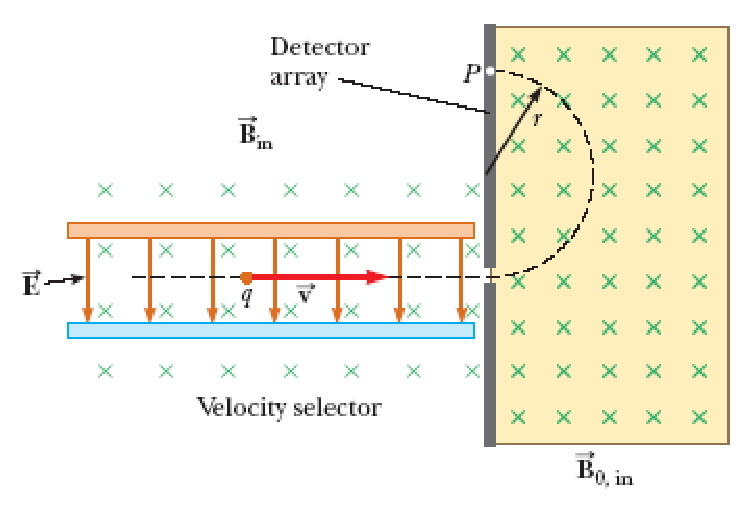
\includegraphics[scale=.42]{MassSpec.eps}
				\caption{Sector mass analyzer with velocity selector}
			\end{figure}
		\end{center}
	\end{frame}
	
	\subsection{Cubic Ion Trap}
	\begin{frame}[c]{Cubic Ion Trap}
		\begin{center}
			\begin{figure}
				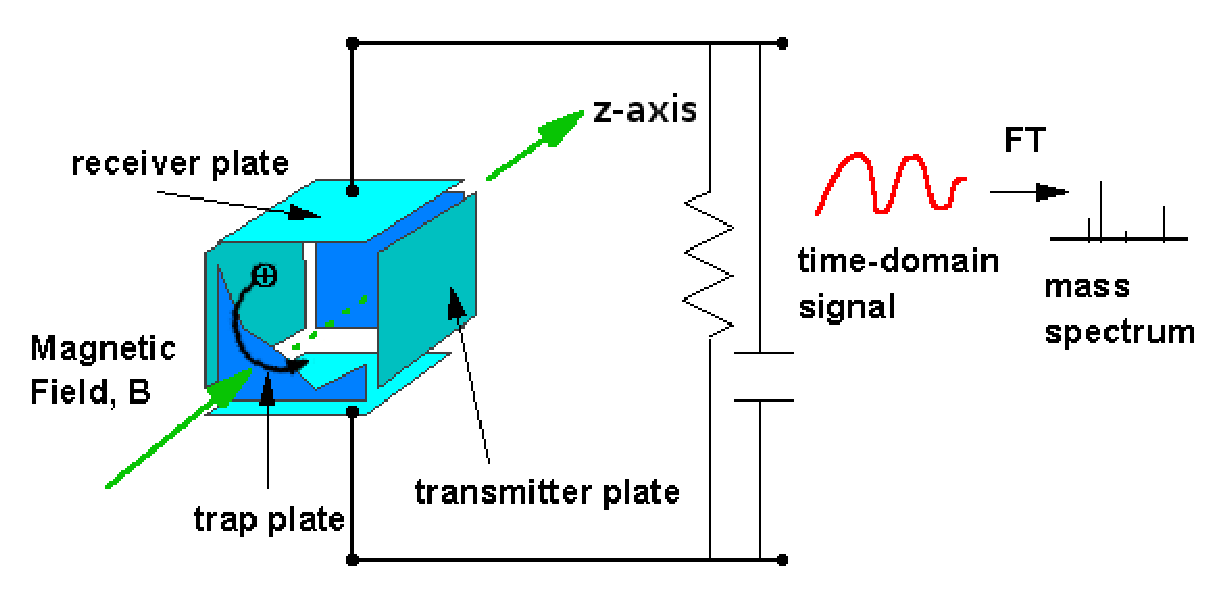
\includegraphics[scale=.42]{schematic_fixed.eps}
				\caption{Diagram of FT-ICR Mass Spectrometer. [http://www.chem.ucsb.edu/\textasciitilde devries/groupsite/labicr.htm]}
			\end{figure}
		\end{center}
	\end{frame}
	
	\subsection{Simplified Motion}
	\begin{frame}[c]{Ion Cyclotron Motion}
		\begin{columns}
			\begin{column}{5cm}
				\vspace{-1cm}
				\begin{center}
					Perspective of $x$-$y$ plane \\[4pt]
				\end{center}
				%\psset{unit=1cm}
				\begin{pspicture*}(-2.2,-2.2)(5,2.5)
					%\psaxes[labels=none](0,0)(-7,-3)(7,3)        % sets up axis
					\pnode(0,0){ori}
					\pnode(0,2){ion}
					\pnode(0,2.2){ion_t}
					\pnode(0,1.8){ion_b}
					\pnode(-.2,2){ion_l}
					\pnode(.2,2){ion_r}
						
					\pnode(-1.5,2){tangent}
					\pnode(0,.5){radial}
						
					\pnode(3,0){B}
					\pnode(2.75,.25){B_tl}
					\pnode(3.25,.25){B_tr}
					\pnode(2.75,-.25){B_bl}
					\pnode(3.25,-.25){B_br}
				
					\pscircle[linewidth=2pt](ori){2}
						
					\psline[linewidth=2pt, linecolor=blue]{->}(ion)(tangent)
					\uput[-135](tangent){\large$\bf v$} 
					\psline[linewidth=2pt, linecolor=blue]{->}(ion)(radial)
					\uput[-45](radial){\large$\bf q\,v\,B_0$}  
						
					\pscircle*[linecolor=white](ion){.4}
					\pscircle[linewidth=2pt](ion){.4} 
					\psline[linewidth=2pt](ion_b)(ion_t)
					\psline[linewidth=2pt](ion_r)(ion_l)
					
					\pscircle[linewidth=2pt](B){.35355}
					\psline[linewidth=2pt](B_tl)(B_br)
					\psline[linewidth=2pt](B_bl)(B_tr)
					\uput[-125](B_br){\large$\bf B_0$}   
				\end{pspicture*} \pause
			\end{column}
			\begin{column}{5cm}
				\begin{overprint}
					Ion cyclotron frequency \\
					$$\boxed{\omega=\frac{q\,B_0}{m}}$$ \pause
					\begin{itemize} \itemsep2pt
						\item Unique frequency $\omega$ for every $\frac{m}{q}$
						\item Independent of initial velocity
					\end{itemize}				
				\end{overprint}
			\end{column}
		\end{columns}
	\end{frame}
	
	\begin{frame}[c]{Trapping oscillation}
		\begin{center}
			Perspective of $z$-axis \\[4pt]
		\end{center}
		\begin{pspicture*}(-5.5,-1.5)(5.5,1.5)
			\psaxes[labels=none](0,0)(-4,0)(4,0)       % sets up axis
			\uput[-90](0,0){$0$} 
			
			\pnode(-4,1){topleftplate}
			\pnode(-4,-1){botleftplate}
			\pnode(4,1){toprightplate}
			\pnode(4,-1){botrightplate}
			\psline[linewidth=2pt, linecolor=black]{-}(topleftplate)(botleftplate)
			\uput[-135](topleftplate){\large$\bf -d/2$} 
			\psline[linewidth=2pt, linecolor=black]{-}(toprightplate)(botrightplate)
			\uput[-45](toprightplate){\large$\bf d/2$} 
			
			\pnode(1.5,0){ion}
			\pnode(1.5,.1){ion_t}
			\pnode(1.5,-.1){ion_b}
			\pnode(1.4,0){ion_l}
			\pnode(1.6,0){ion_r}
			\uput[70](.75,0){$a$} 
			\psline[linewidth=2.5pt, linecolor=red]{->}(ion)(.75,0)
			\uput[110](2.5,0){$v$} 
			\psline[linewidth=2.5pt, linecolor=green]{->}(ion)(2.5,0)
			\pscircle*[linecolor=white](ion){.2}
			\pscircle[linewidth=1.25pt](ion){.2}
			\psline[linewidth=1.5pt](ion_b)(ion_t)
			\psline[linewidth=1.5pt](ion_r)(ion_l)
			
			\uput[120](-3,0){$E_1$} 
			\psline[linewidth=3pt, linecolor=blue]{->}(-4,0)(-3,0)
			\uput[60](3,0){$E_2$}
			\psline[linewidth=3pt, linecolor=blue]{->}(4,0)(3,0)
			
			%\psline[linewidth=1.25pt, linecolor=black](nhalf_d)(half_d)
	
			%\pscircle[linewidth=2pt](ori){2}
			%\psline[linewidth=2pt, linecolor=blue]{->}(ion)(radial)
			%\uput[45](B_tr){\large$\bf B_0$}   
		\end{pspicture*}
		Electric Field in Z-direction: \\[6pt]
		$$E(z)= -k\,z\qquad\text{where}\qquad k=\frac{4V_t}{d^2}$$
	\end{frame}
	
	\begin{frame}[c]{Excitation \& Detection}
		\begin{columns}
			\begin{column}{5cm}
				Excitation of specific ion:
				$$E(t)=E_0\,\cos(\omega_0\,t)\,y$$
				\vspace{.25cm}
				Detected potential voltage:
				$$\frac{1}{\frac{d}{2}-x}-\frac{1}{\frac{d}{2}+x}$$
			\end{column}
			\begin{column}{5cm}
				\begin{overprint}
					\vspace{-1mm}
					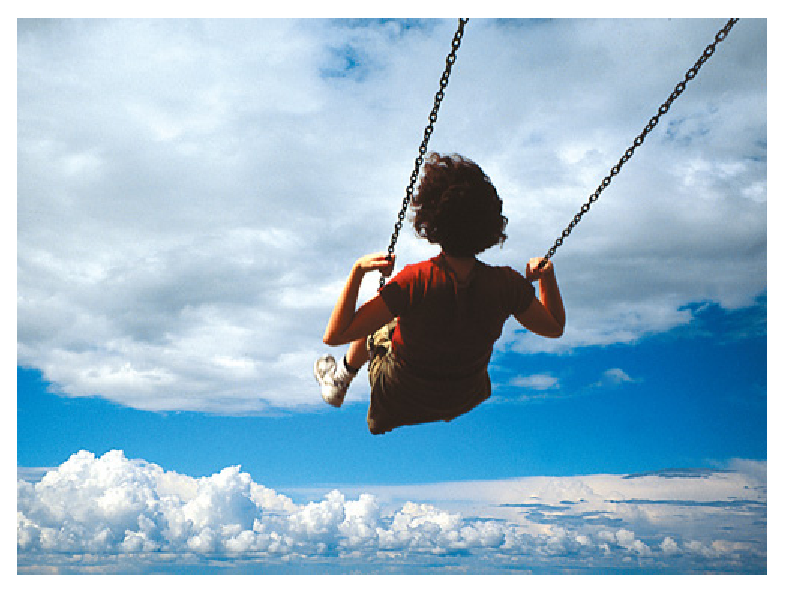
\includegraphics[scale=.42]{swinghigh.eps}
				\end{overprint}
			\end{column}
		\end{columns}
	\end{frame}
	
	\section{EJS}
	\begin{frame}[c]{Easy Java Simulations}
		\begin{itemize} \itemsep4pt
			\item Free tool to generate Java Simulations
			\item Built-in ODE editor and solvers
		\end{itemize}
		\vspace{.25cm}
		\begin{center}
			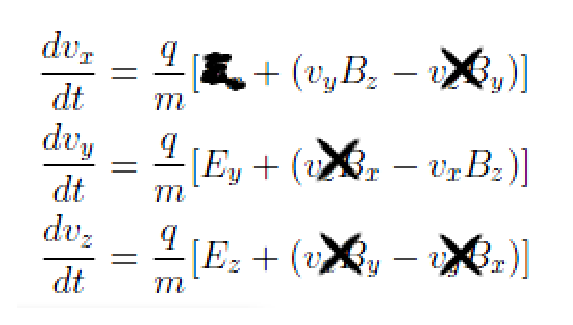
\includegraphics[scale=.5]{eqn4_simplied.eps}
		\end{center}
	\end{frame}
		
	\section{Close}

	\subsection{References}
	\begin{frame}[allowframebreaks]{References}
		\footnotesize
		\nocite{*}
		\bibliographystyle{IEEEtran}
		\bibliography{fourier_transforms}
	\end{frame}

	\subsection{Acknowledgements}
	\begin{frame}[c]{Acknowledgements}
		\begin{itemize} \itemsep5pt
			\item Dr Hightower, Dr K Titus, Dr A Titus, and Dr DeWitt
			\item Classmates and others for random questions
		\end{itemize}
	\end{frame}
	
	\subsection{Question} 
	\begin{frame}[c]{Question}
		
\includegraphics[scale=.42]{questions.eps}
	\end{frame}
	
\end{document}